% This is a basic Math Paper

\documentclass[11pt]{article}

% Preamble

\usepackage[margin=1in]{geometry}
\usepackage{amsfonts, amsmath, amssymb}
\usepackage{gensymb}
\usepackage{fancyhdr, float, graphicx}
\usepackage[utf8]{inputenc} % Required for inputting international characters
\usepackage[T1]{fontenc} % Output font encoding for international characters
\usepackage{fouriernc} % Use the New Century Schoolbook font
\usepackage[nottoc, notlot, notlof]{tocbibind}


% Header and Footer
\pagestyle{fancy}
\fancyhead{}
\fancyfoot{}
\fancyhead[L]{\textit{\Large{Engineering Mechanics Experiment 9}}}
%\fancyhead[R]{\textit{something}}
\fancyfoot[C]{\thepage}
\renewcommand{\footrulewidth}{1pt}



% Other Doc Editing
% \parindent 0ex
%\renewcommand{\baselinestretch}{1.5}

\begin{document}
	
	\begin{titlepage} 
		\centering 
		
		%---------------------------NAMES-------------------------------
		
		\huge\textsc{
			MIT World Peace University
		}\\
	
		\vspace{0.75\baselineskip} % space after Uni Name
		
		\LARGE{
			Engineering Mechanics\\
			First Year B. Tech, Trimester 1
		}
	
		
		\vfill % space after Sub Name
		
		%--------------------------TITLE-------------------------------
		
		\rule{\textwidth}{1.6pt}\vspace*{-\baselineskip}\vspace*{2pt}
		\rule{\textwidth}{0.6pt}
		\vspace{0.75\baselineskip} % Whitespace above the title
		
		
		
		\huge{\textsc{
				Graphical representation of Problems involving Rectilinear Motion and Motion Curves
			}} \\
		
		
		
		\vspace{0.5\baselineskip} % Whitespace below the title
		\rule{\textwidth}{0.6pt}\vspace*{-\baselineskip}\vspace*{2.8pt}
		\rule{\textwidth}{1.6pt}
		
		\vspace{1\baselineskip} % Whitespace after the title block

		%--------------------------SUBTITLE --------------------------	
			
		\LARGE\textsc{
			Experiment 10\\
			Practical Report
		} % Subtitle or further description
		\vfill
		
		%--------------------------AUTHOR-------------------------------
		
		Prepared By
		\vspace{0.5\baselineskip} % Whitespace before the editors
		
		\Large{
			Krishnaraj Thadesar \\
			Division 9, Roll No. 54
		}
		
		
		\vspace{0.5\baselineskip} % Whitespace below the editor list
		\today

	\end{titlepage}
	
	
\tableofcontents
\thispagestyle{empty}
\clearpage


\setcounter{page}{1}

\section{Objective}
To find Graphically and Analytically the resultant of a set of problems involving Rectilinear Motion and Motion Curves, and to compare the results thereby finding the Percentage Error.

\section{Theory}
The Following laws and concepts have been used in this experiment.

\subsection{Velocity}
The velocity of an object is the rate of change of its position with respect to a frame of reference, and is a function of time. Velocity is equivalent to a specification of an object's speed and direction of motion (e.g. 60 km/h to the north).

\subsection{Acceleration}
In mechanics, acceleration is the rate of change of the velocity of an object with respect to time. Accelerations are vector quantities (in that they have magnitude and direction).

\subsection{Equations of Motion}
In physics, equations of motion are equations that describe the behavior of a physical system in terms of its motion as a function of time. More specifically, the equations of motion describe the behavior of a physical system as a set of mathematical functions in terms of dynamic variables. These variables are usually spatial coordinates and time.\\

The Equations used here are applicable to uniformly accelerated motion. 

\begin{equation}
	\begin{aligned}
		&v=u+a t \\
		&s=u t+\frac{1}{2} a t^{2} \\
		&v^{2}=u^{2}+2 a s
	\end{aligned}
\end{equation}

\subsection{Distance Time Graph}
A distance-time graph shows how the distance and speed of an object changes with time. This graph shows the movement of three objects over time. The slope, or steepness, of each line indicates the object's rate of speed. In general, the steeper the slope, the faster the object's speed. A straight line indicates constant speed, whereas changes in slope at different time intervals indicate changing speeds.

\begin{figure}[H]
	\centering
	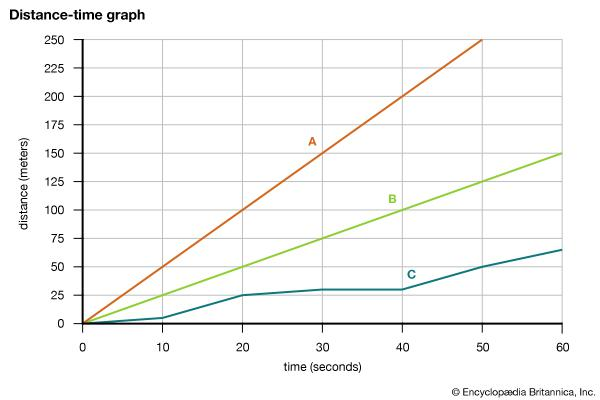
\includegraphics[scale=0.5]{st graph.jpg}
	\caption{Distance Time Graph}
\end{figure}


The Slope of a Distance time graph is the velocity.

$$ \mathrm{Velocity}\ v = \frac{Distance}{Time} $$

Instantaneous Velocity can be found as:

\begin{equation}
	v(t)=\lim _{\Delta t \rightarrow 0} \frac{x(t+\Delta t)-x(t)}{\Delta t}=\frac{d x(t)}{d t}
\end{equation}

\subsection{Velocity Time Graph}
The velocity of an object is its speed in a particular direction. Two cars travelling at the same speed but in opposite directions have different velocities. A velocity-time graph shows the speed and direction an object travels over a specific period of time. Velocity-time graphs are also called speed-time graphs. The vertical axis of a velocity-time graph is the velocity of the object. The horizontal axis is the time from the start.1

\begin{figure}[H]
	\centering
	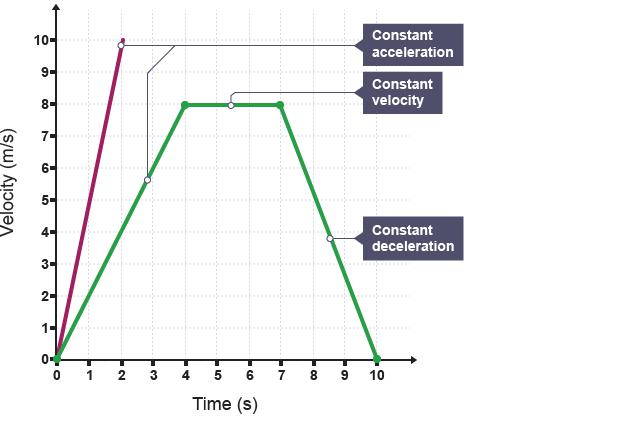
\includegraphics[scale=0.45]{vt graph.jpg}
\end{figure}

\noindent
The Slope of the velocity time graph shows the Acceleration.

\begin{equation}
	a(t)=\frac{d}{d t} v(t)
\end{equation}

\subsection{Acceleration Time Graph}
The acceleration time graph is the graph that is used to determine the change in velocity in the given interval of the time. In the acceleration vs time graph on the x-axis you have the time taken by the object and on the y-axis acceleration of the object, in which the area under the graph gives you the change in velocity of the object over the given period of the time. The acceleration time graph is used to find the change in the velocity of the moving object for the given period of time and this can be determined by finding the area under the curve.

\begin{figure}[H]
	\centering
	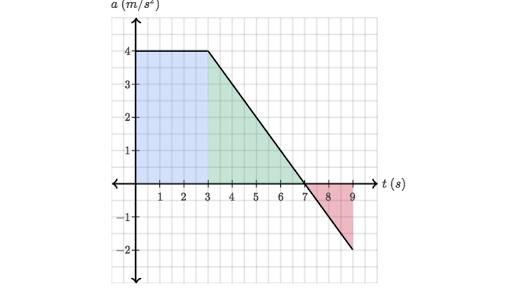
\includegraphics[scale=0.5]{at graph.jpg}
	\label{fig: Polygon Law}
\end{figure}

Distance under the Acceleration Time graph gives the velocity

$$ v = a \times t $$

\section{Procedure}
\begin{enumerate}
	\item Solve the Given Question analytically.
	\item Solve the Given Question Graphically.
	\item Tabulate the Results
	\item Calculate the Error using the Formula
	
		$$\mathrm{Percentage\ Error\ (\eta)} = \dfrac{|\mathrm{Graphical\ Value} - \mathrm{Analytical\ Value}|}{\mathrm{Analytical\ Value}} * 100$$
\end{enumerate}
\pagebreak
\section{Analytical Method}


Q1. A car starting from rest moves along a straight track with an acceleration shown in the Figure. Determine the time t for the car to reach a speed of 50 m/s and construct the v-t diagram that describes the motion until the time 't'.
\begin{figure}[H]
	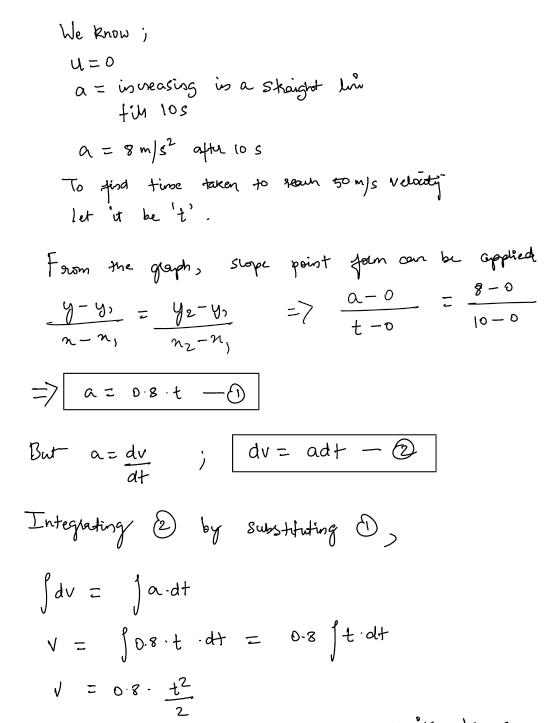
\includegraphics[scale=0.7]{a11.jpg}
	\label{fig: Polygon Law}
\end{figure}

\begin{figure}[H]
	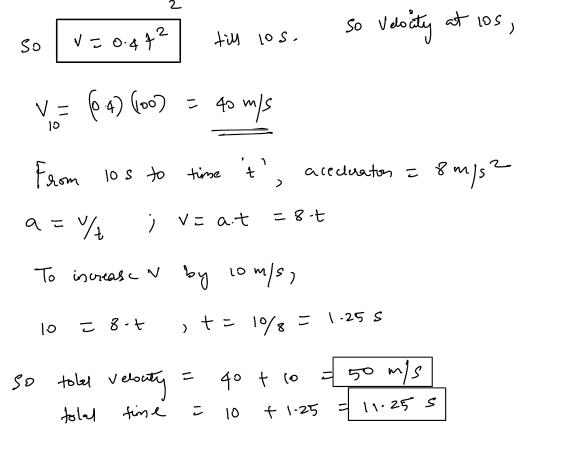
\includegraphics[scale=0.8]{a12.jpg}
	\label{fig: Polygon Law}
\end{figure}

\pagebreak
Q2. A particle moves in a straight line with the acceleration shown in the figure. If $x = -540m$ and $v = 60m/s$ and $t = 0$ then find the total distance travelled by by the particle when $t = 50s$.

\begin{figure}[H]
	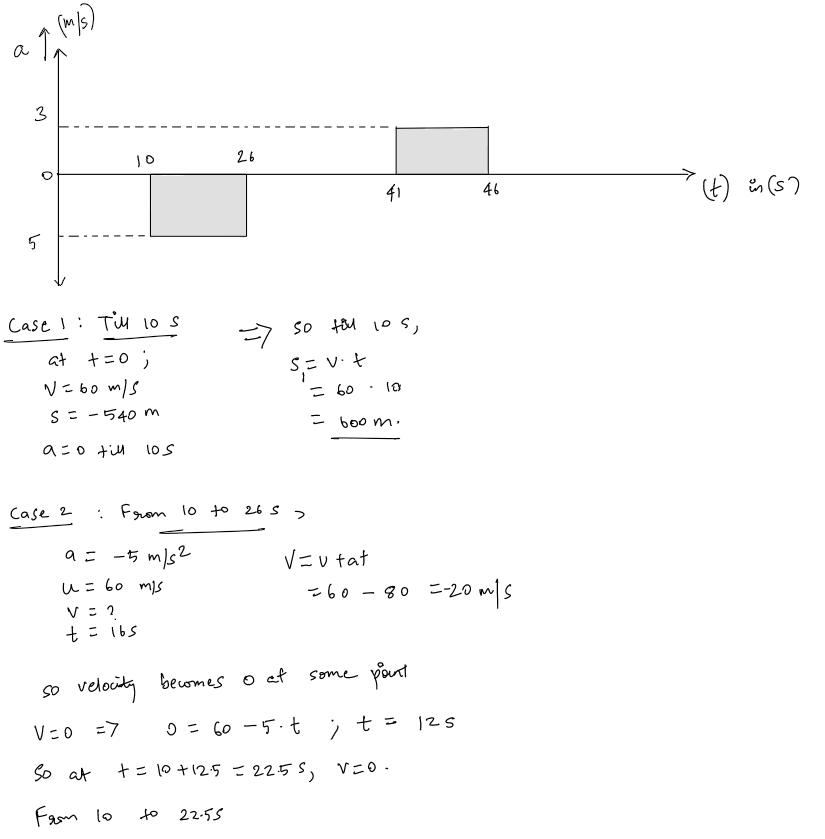
\includegraphics[scale=0.7]{a21.jpg}
	\label{fig: Polygon Law}
\end{figure}

\begin{figure}[H]
	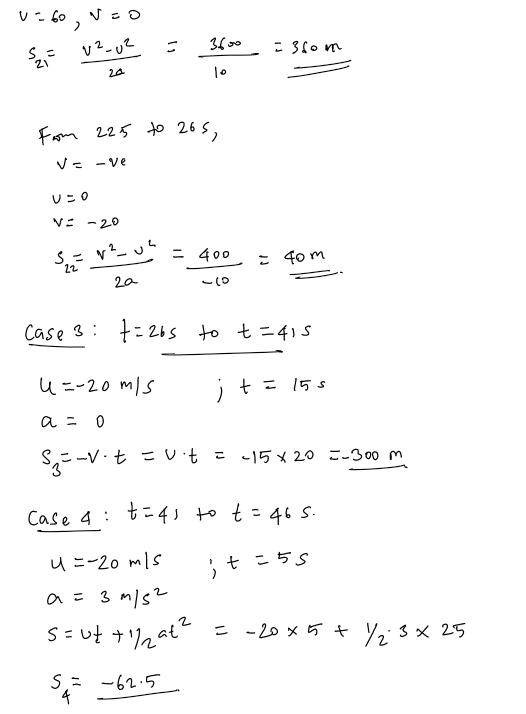
\includegraphics[scale=0.55]{a22.jpg}
	\label{fig: Polygon Law}
\end{figure}


\begin{figure}[H]
	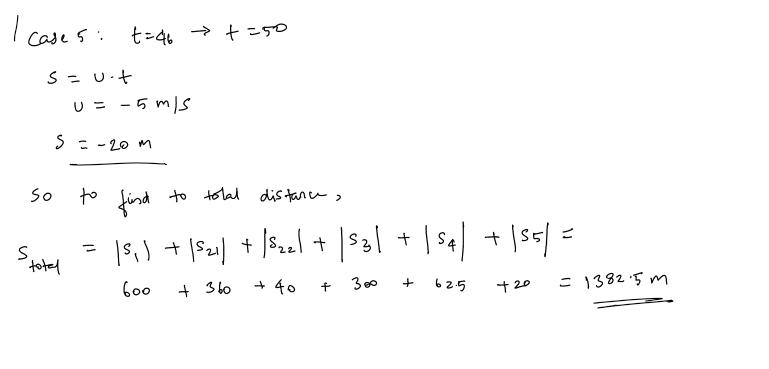
\includegraphics[scale=0.55]{a23.jpg}
	\label{fig: Polygon Law}
\end{figure}
\pagebreak

\section{Graphical Method}
Q1. A car starting from rest moves along a straight track with an acceleration shown in the Figure. Determine the time t for the car to reach a speed of 50 m/s and construct the v-t diagram that describes the motion until the time 't'.
\begin{figure}[H]
	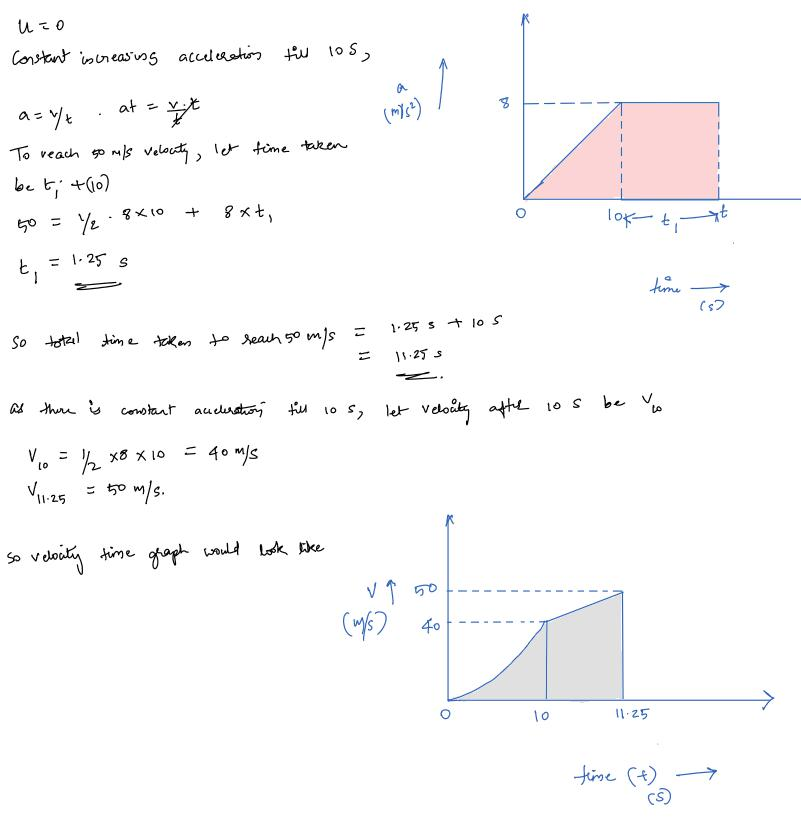
\includegraphics[scale=0.65]{g1.jpg}
	\label{fig: Polygon Law}
\end{figure}


\pagebreak
Q2. A particle moves in a straight line with the acceleration shown in the figure. If $x = -540m$ and $v = 60m/s$ and $t = 0$ then find the total distance travelled by by the particle when $t = 50s$.
\begin{figure}[H]
	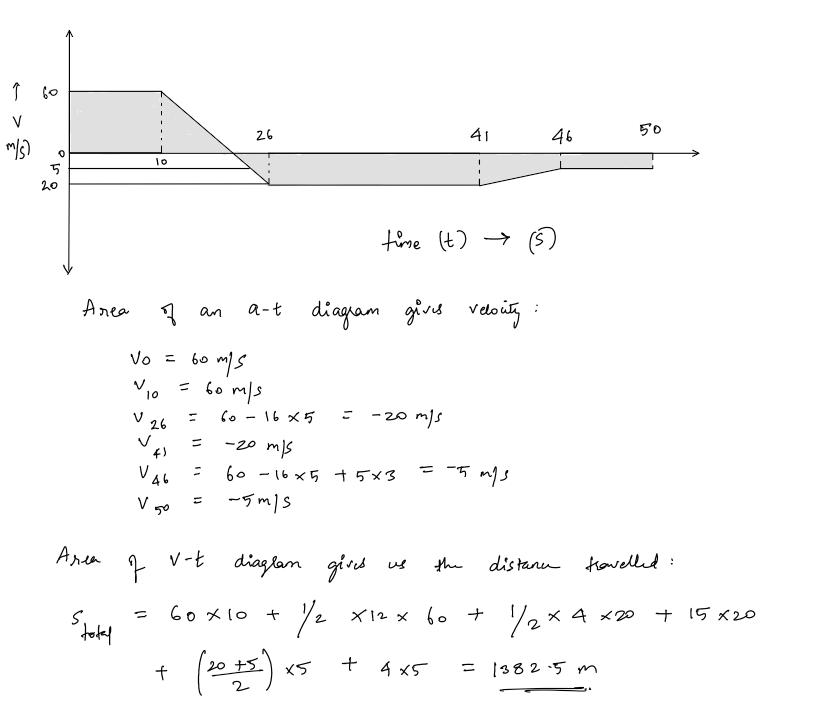
\includegraphics[scale=0.7]{g2.jpg}
	\label{fig: Polygon Law}
\end{figure}

\pagebreak

Q3. The $s-t$ curve for a train travelling along a straight track has been experimentally determined. From the data construct the $ v-t $ and $ a-t $ curve for the motion from $ 0\ to\ 60 $ Seconds. From $ 0\ to\ 30 $ seconds the curve is $ s = (0.4 t^2)m $ where t is in s. 
\begin{figure}[H]
	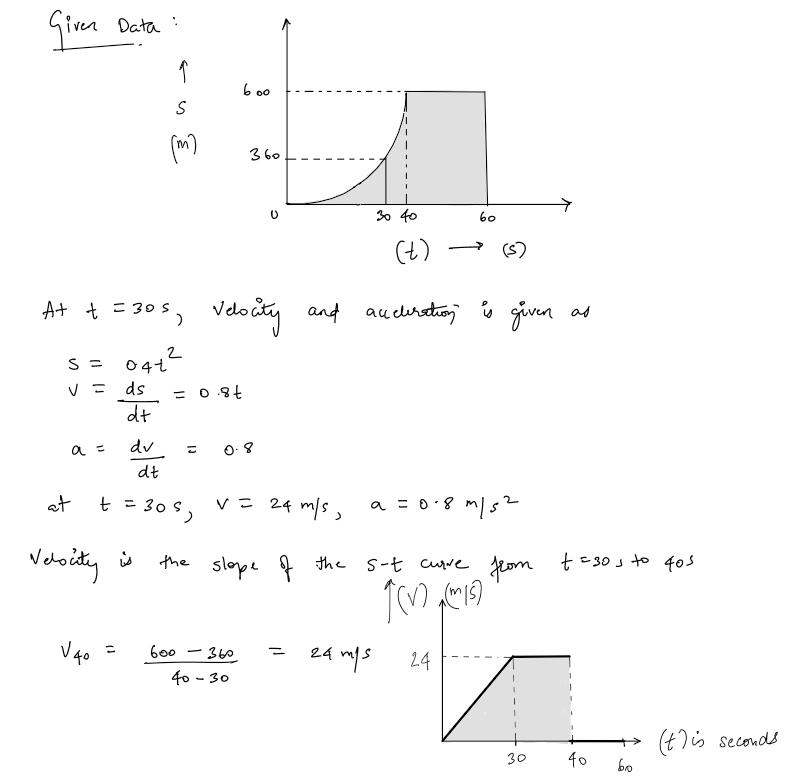
\includegraphics[scale=0.7]{g31.jpg}
	\label{fig: Polygon Law}
\end{figure}
\begin{figure}[H]
	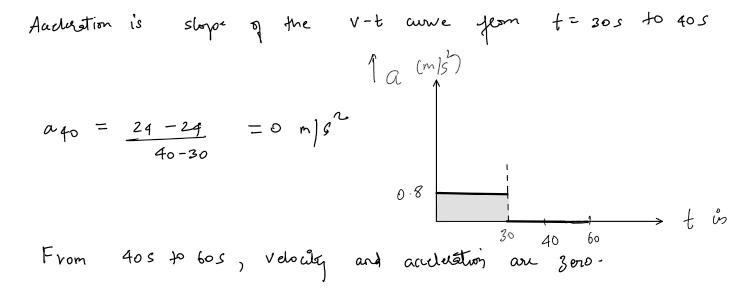
\includegraphics[scale=0.6]{g32.jpg}
	\label{fig: Polygon Law}
\end{figure}
\pagebreak

\section{Results}

\begin{tabular}{|c|c|c|c|}
	\hline
	Question Number & Analytical Solution & Graphical Solution & Percent Error \\
	\hline
	1 	& t = 11.25s  & t = 11.25s & $\eta_t = 0\%$\\
	\hline
	2 	& x = 1382.5m  & x = 1382.5 & $\eta_x = 0\%$ \\
	\hline
\end{tabular}


\section{Conclusion}
A set of problems involving Rectilinear Motion and Motion Curves were solved using graphical as well as analytical methods. The Percentage error between the two answers was found.
\end{document}